\chapter{Desempenho}

\section{Atualização da Estimativa de Peso}

Devido a alteração das empenagens, uma nova análise de peso foi realizada utilizando os métodos propostos por Shevell \cite{shevell1989fundamentals} na compania Douglas Aircraft e Kroo \cite{kroo_shevell} por meio do software SUAVE \cite{lukaczyk2015suave,SUAVE}. As equações para estimativa de peso dos componentes são apresentadas abaixo de acordo com a referência \cite{lukaczyk2015suave}:

\begin{enumerate}
\item \textbf{Asa}

\begin{equation}
W_{wing} = 4.22 S_{w} + 1.642 \cdot 10^{-6} \cdot \frac{  N_{ult} b^3 \sqrt{W_{MTOW} W_{MZF}} (1 + 2\cdot \lambda) }{(t/c)_{avg} \cos{\Lambda_{c/4}}^2 S_w (1+\lambda) }
\end{equation}

\begin{description}
\item [$W_{wing}$ -] Wing structural weight
\item [$S_{w}$ -] Wing area
\item [$N_{ult}$ -] Ultimate design load factor for the aircraft. Its value must comply with aeronautical regulations such as CFR 14 Part 25.
\item [$b$ -] Wing span
\item [$\lambda$ -] Wing taper ratio
\item [$(t/c)_{avg}$ -] Wing thickness to chord ratio
\item [$\Lambda_{c/4}$ -] Wing sweep angle at $1/4$ chord line
\end{description}

\vspace{0.5cm}

\item \textbf{Empenagem Horizontal + Profundor}

\begin{equation}
W_{HT} = 5.25 S_{HT} + 0.8 \cdot 10^{-6} \cdot \frac{ N_{ult} b_{HT}^3 W_{MTOW} c_w \sqrt{S_{HT}} } { (t/c)_{avg} \cos{\Lambda_{HT_{c/4}}}^2  l_{HT} S_{HT}^{1.5}}
\end{equation}

\begin{description}
\item [$W_{HT}$ -] Horizontal Tail structural weight
\item [$S_{HT}$ -] Horizontal Tail area
\item [$b_{HT}$ -] Horizontal Tail span
\item [$l_{HT}$ -] Distance between wing aerodynamic center and horizontal tail aerodynamic center
\item [$(t/c)_{avg}$ -] Horizontal Tail thickness to chord ratio
\item [$\Lambda_{HT_{c/4}}$ -] Horizontal Tail sweep angle at $1/4$ chord line
\end{description}

\vspace{0.5cm}

\item \textbf{Empenagem Vertical}

\begin{equation}
W_{VT} = 2.62 S_{VT} + 1.5 \cdot 10^{-5} \cdot \frac{ N_{ult} b_{VT}^3 \left( 8.0 + 0.44 \cdot \frac{W_{MTOW}}{S_w} \right)  }{  (t/c)_{avg} \cos{\Lambda_{VT_{c/4}}}^2 }
\end{equation}

\begin{description}
\item [$W_{vT}$ -] Vertical Tail and Elevator structural weight
\item [$S_{vT}$ -] Vertical Tail area
\item [$b_{vT}$ -] Vertical Tail span
\item [$(t/c)_{avg}$ -] Vertical Tail thickness to chord ratio
\item [$\Lambda_{VT_{c/4}}$ -] Vertical Tail sweep angle at $1/4$ chord line
\end{description}

\vspace{0.5cm}

\item \textbf{Fuselagem}

\begin{equation}
I_p = 1.5 \cdot 10^{-3} \Delta P_f \cdot w_f
\end{equation}

\begin{equation}
I_b = 1.91 \cdot 10^{-4} \cdot N_{lim} (W_{MZF} - W_w - W_{w,p}) \cdot \frac{l_{f,e}}{h_f^2}
\end{equation}

If the $I_p >\;I_b$, $I_f = I_p$. If not,

\begin{equation}
I_f = \frac{I_p^2+I_b^2}{2\cdot I_b}
\end{equation}

\begin{equation}
W_f = (1.051+1.020 \cdot I_f) S_{f,wetted}
\end{equation}

\begin{description}
\item [$W_f$ -] Fuselage structural weight
\item [$\Delta P_f$ -] Maximum pressure differential of the fuselage
\item [$W_{w,p}$ -] Weight of the wing-mounted engines, nacelles and pylons
\item [$l_{f,e}$ -] Effective fuselage length. Fuselage length minus the wing chord root divided by two.
\item [$h_f$ -] Fuselage Height
\end{description}

\vspace{0.5cm}

\item \textbf{Diversos}

Para aeronaves com 300 assentos ou menos,

\begin{equation}
W_{furn} = (43.7 - 0.037 \cdot N_{seat} ) + 46 \cdot N_{seat}
\end{equation}

Para aeronaves com mais de 300 passageiros,

\begin{equation}
W_{furn} = (43.7 - 0.037 \cdot 300 ) + 46 \cdot N_{seat}
\end{equation}

\begin{description}
\item [$W_{furn}$ -] Peso
\item [$N_{seat}$ -] Numero de passageiros
\end{description}

\vspace{0.5cm}

\item \textbf{Trem de Pouso}

\begin{equation}
W_{LG} =  0.04 \cdot W_{MTOW}
\end{equation}

\begin{description}
\item [$W_{LG}$ -] Landing Gear Weight
\end{description}

\vspace{0.5cm}

\item \textbf{Sistema Propulsivo}

\begin{equation}
W_{propulsion} = 1.6 \cdot W_{p,dry} = 1.6 \cdot (0.4054 \cdot T_{SLS}^{0.9255})
\end{equation}

\begin{description}
\item [$W_{propulsion}$ -] Propulsion system Weight
\item [$W_{p,dry}$ -] Dry weight of the engine
\item [$T_{SLS}$ -] Sea-level static thrust
\end{description}

\end{enumerate}



A estimativa final de peso é apresentada e comparada com a aeronave ATR42-500 na tabela abaixo :

\begin{table}[H]
    \centering
    \begin{tabular}{cc}
    \toprule
    Componente & Peso ($kg$) \\ \midrule
    Empenagem Horizontal & 233 \\
    Propulsão & 1760 \\
    Leme de Direção & 77 \\
    Sistemas & 4492 \\
    Fuselagem & 2216 \\
    Trem de Pouso & 768 \\
    Empenagem Vertical & 191 \\
    Asa & 2094 \\ \midrule
    Peso Vazio & 11830 \\
    ATR 42-500 & 11250 \\ \midrule
    Diferença  & 580 \\
    \bottomrule
    \end{tabular}
    \caption{Peso Vazio da Aeronave}
    \label{tab:results_weight}
\end{table}

A Diferença de peso é justificada pela fuselagem mais pesada devido ao comprimento maior. Por fim, os pesos de projeto da aeronave foram definidos como:

\begin{table}[H]
    \centering
    \begin{tabular}{cc}
    \toprule
       & Peso ($kg$) \\ \midrule
    MTOW & 19200 \\
    MZFW & 17130 \\
    Carga Paga Máxima & 5300 \\
    Máximo combustível & 4500 \\
    BOW & 11830 \\
    \bottomrule
    \end{tabular}
    \caption{Peso Vazio da Aeronave}
    \label{tab:weight}
\end{table}


\section{Missão Típica}

A missão típica da aeronave é baseada na tabela e figura abaixo e nos requistos dimensionantes apresentados no \autoref{diagramarestricoes}.

\begin{table}[H]
\centering
\begin{tabular}{clcl}
\toprule
0-1 & Taxi & 4-5 & Descida (Descent) \\
1-2 & Decolagem (Take-off) & 5-6 & Loiter \\
2-3 & Subida (Climb) & 6-7 & Pouso (Landing) \\
3-4 & Cruzeiro (Cruise) & 7-0 & Taxi \\
\bottomrule
\end{tabular}
\caption{Segmentos de uma missão típica comercial}
\label{tbl:mission_segments}
\end{table}


\begin{figure}[H]
\centering
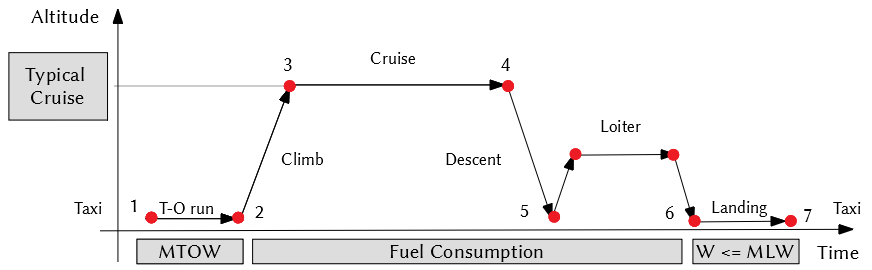
\includegraphics[width=130mm]{images/parte4/missao_tipica_generica.PNG}
\caption{Missão Típica}
\label{fig:typical_mission}
\end{figure}

A aeronave, juntamento com o motor PW127, foi modelada no software SUAVE para simulação da missão considerando os segmentos apresentados acima. A entrada do programa é a geometria da aeronave e o perfil de missão desejado. O software divide cada segmento em pontos em que as equações de movimento serão integradas, além disso, é importante destacar que o SUAVE não modela o transitório de um segmento para o outro, dessa forma, os gráficos dos estados do avião pode apresentar discontinuidades que não afetam a estimativa de desempenho da aeronave. A tabela abaixo resume o perfil de missão implementado no SUAVE sendo o alcance da missão de projeto (segmento 0 a 5) de 750 nm para número máximo de passageiros (5000 kg de carga paga):

\begin{table}[H]
\centering
\begin{tabular}{clc}
\toprule
    & Segmento & Descrição \\
0-1 & Taxi & MTOW + combustível para taxi\\
1-2 & Decolagem & MTOW, ISA, nível do mar, flap 15° \\
2-3 & Subida   & $CAS = 170 \; knots$, Manete de potência no máximo, \\
 & & Tempo de subida para FL250 igual a 28 min\\
3-4 & Cruzeiro & $Mach = 0.523$ ou $TAS = 315 \; knots$ a FL250\\
4-5 & Descida  & Razão de descida constante de 2000 ft/min \\
5-6 & Loiter   & 45 min + 100nm de aeroporto alternativo\\
6-7 & Pouso    & ISA, nível do mar, flap 30°\\
7-0 & Taxi     & \\
\bottomrule
\end{tabular}
\caption{Missão Implementada no software SUAVE}
\label{tbl:mission_suave}
\end{table}

O consumo de combustível considerando para reserva foi de 740 kg. O consumo de bloco estimado foi de 1630 kg sendo o total de combustível necessário 2370 kg. Os gráficos abaixo resumem a simulação da missão.

\clearpage

\begin{figure}[H]
\centering
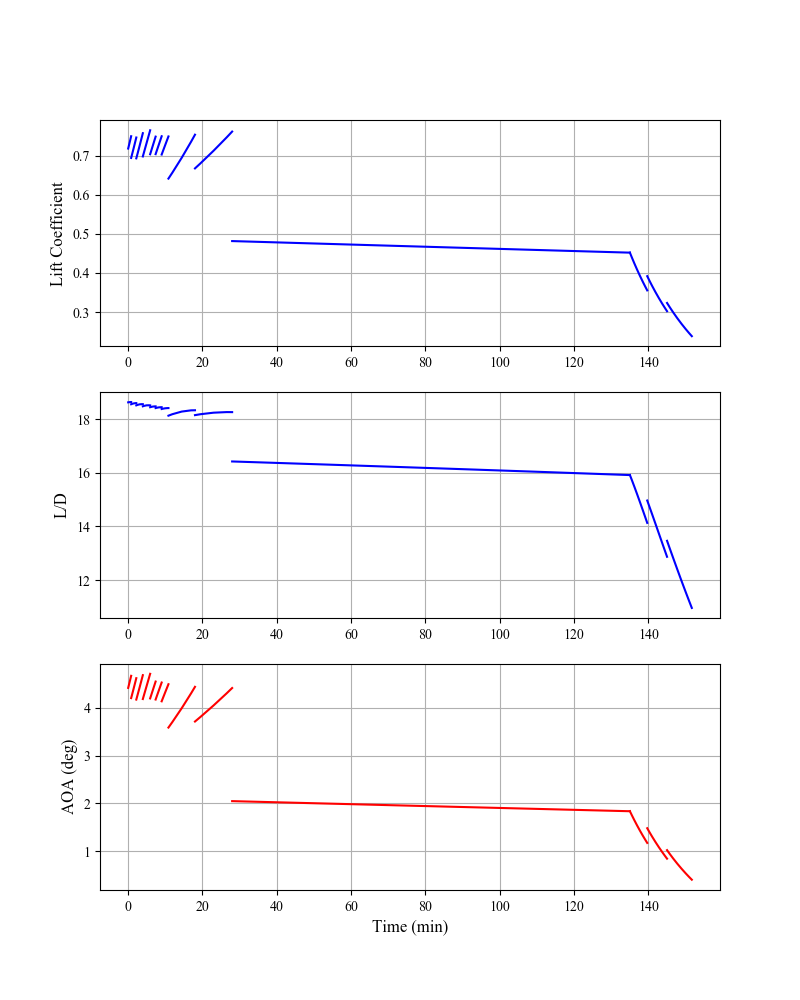
\includegraphics[width=1.\textwidth]{images/parte4/aero0.png}
\caption{Resultado SUAVE para Missão Típica}
\label{fig:aero_mission}
\end{figure}

\begin{figure}[H]
\centering
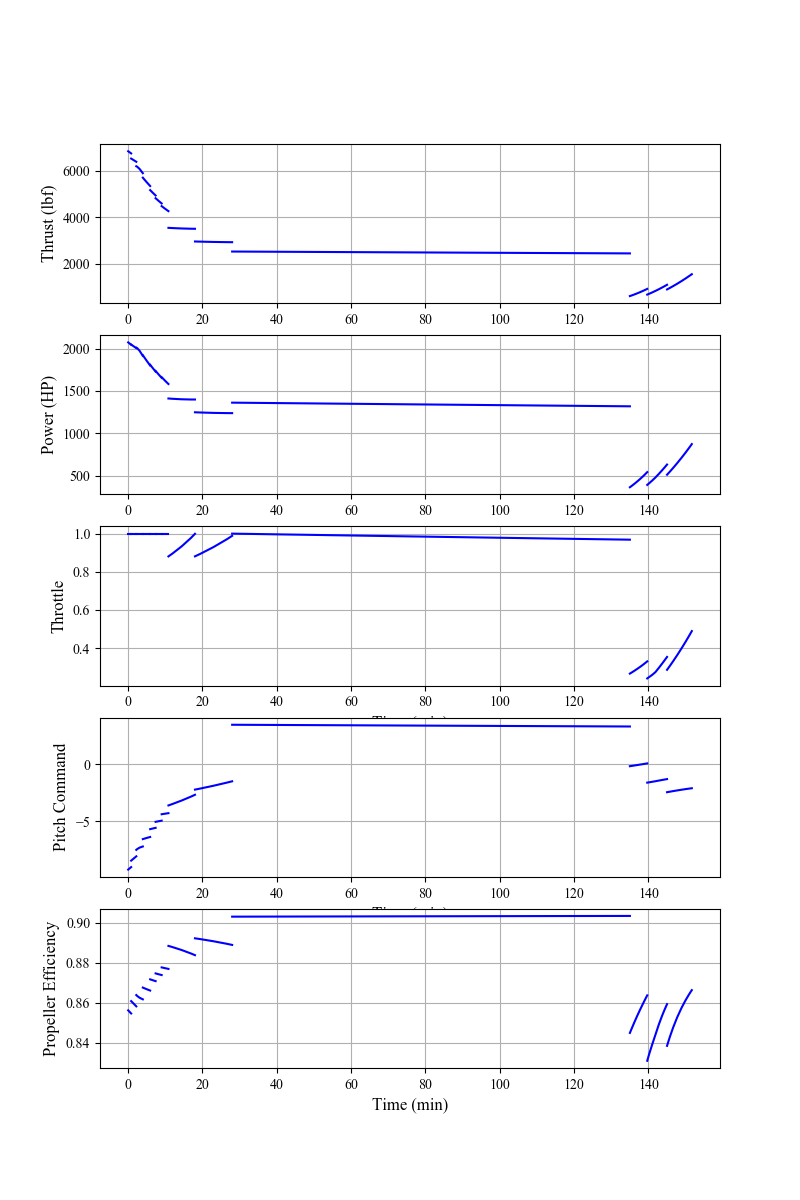
\includegraphics[width=0.95\textwidth]{images/parte4/engine0.png}
\caption{Resultado SUAVE para Missão Típica}
\label{fig:engine_mission}
\end{figure}

\begin{figure}[H]
\centering
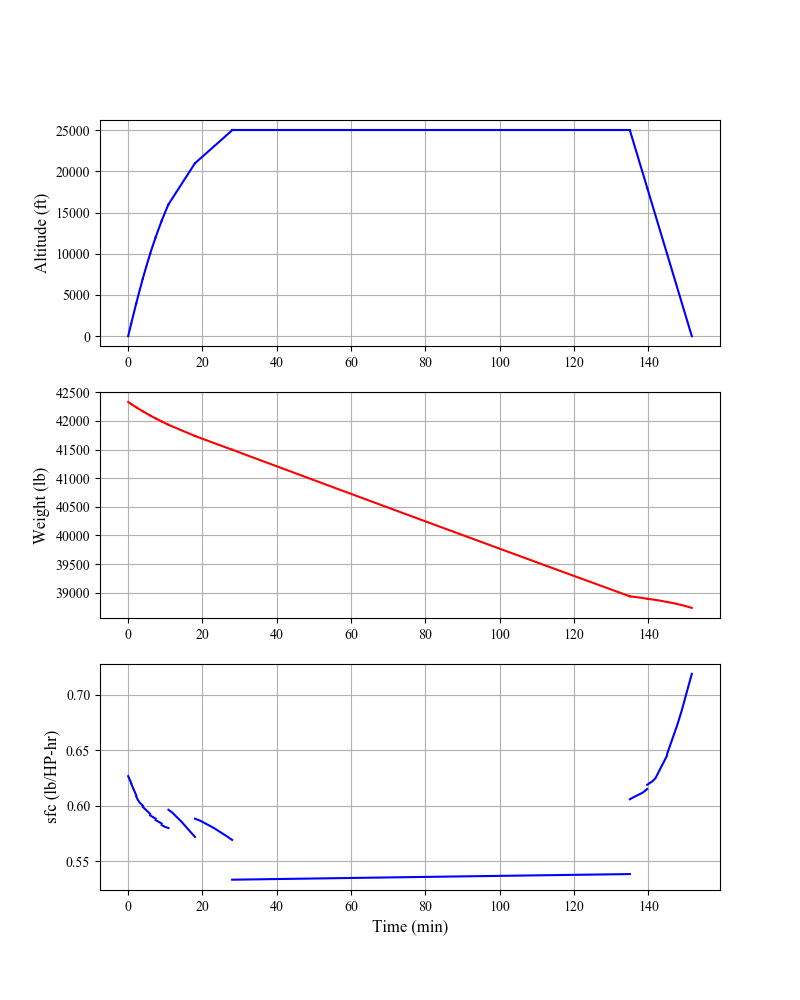
\includegraphics[width=1.\textwidth]{images/parte4/mission0.png}
\caption{Resultado SUAVE para Missão Típica}
\label{fig:mission_mission}
\end{figure}

\begin{figure}[H]
\centering
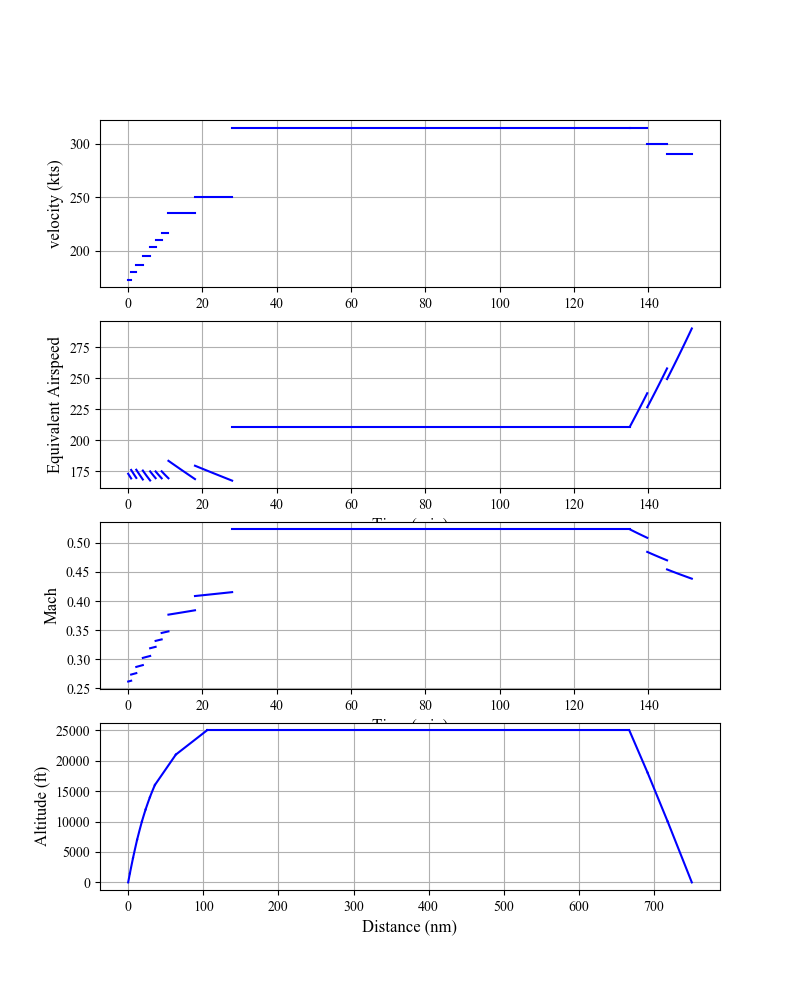
\includegraphics[width=1.\textwidth]{images/parte4/vel0.png}
\caption{Resultado SUAVE para Missão Típica}
\label{fig:vel_mission}
\end{figure}

Com esses resultados, pode-se concluir que a aeronave atende aos requistos dimensionantes estipulados no \autoref{diagramarestricoes} e inclusive supera os valores estipulados para velocidade de cruzeiro.


\section{Diagrama de Carga Paga vs. Alcance}

Com o perfil típico da missão definido, é possível construir o diagrama de carga paga vs alcance que é explicado pela \autoref{fig:payloadrangediagram}

\begin{figure}[H]
\centering
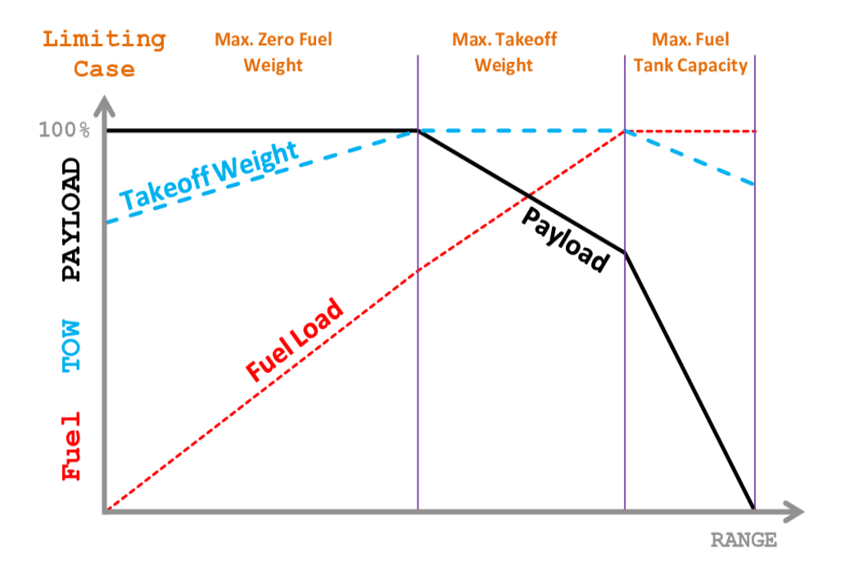
\includegraphics[width=120mm]{images/parte4/payloadrangediagram.png}
\caption{Exemplo de Diagrama de Carga Paga vs. Alcance}
\label{fig:payloadrangediagram}
\end{figure}

Para a aeronave em projeto, o diagrama de carga paga vs alcance é apresentado na \autoref{fig:payloadrange}.

\begin{figure}[H]
\centering
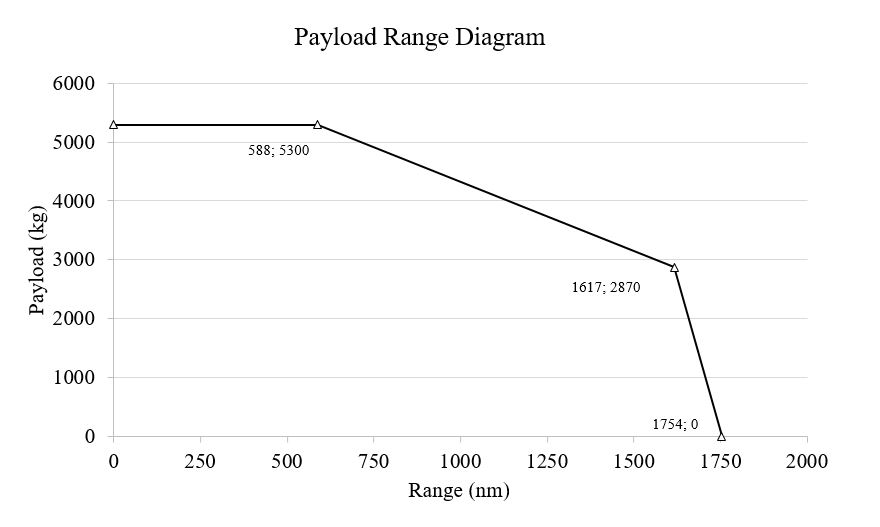
\includegraphics[width=1.\textwidth]{images/parte4/payload_range.JPG}
\caption{Diagrama de Carga Paga vs. Alcance final}
\label{fig:payloadrange}
\end{figure}

\section{Pista de Decolagem}

Para estimativa de pista de Decolagem, utilizou-se o modelo paramétrico proposto por \cite{lukaczyk2015suave} dado pela \autoref{eq:TOFL}.

\begin{equation}
\label{eq:TOFL}
    TOFL = \sum_{i=0}^{2} k_i \cdot \left[ \frac{V_{2}^2}{T/W} \right]^i
\end{equation}


\begin{table}[H]
    \centering
    \begin{tabular}{c|c c c}
        Engine & $k_0$ & $k_1$ & $k_2$  \\ \toprule
         2 & 857.4 & 2.476 & 1.40e-4 \\
         3 & 667.9 & 2.343 & 9.30e-5 \\
         4 & 486.7 & 2.282 & 7.05e-5 \\ \bottomrule
    \end{tabular}
    \caption{Coeficientes da \autoref{eq:TOFL}}
    \label{tab:my_label}
\end{table}

A \autoref{fig:tofl} apresenta os resultados obtidos considerando apenas flaps como superfícies de sustentação, assim como na aeronave ATR 72-600, com uma deflexão de 15° e $C_{L_{max}} = 2.11$.

\begin{figure}[H]
\centering
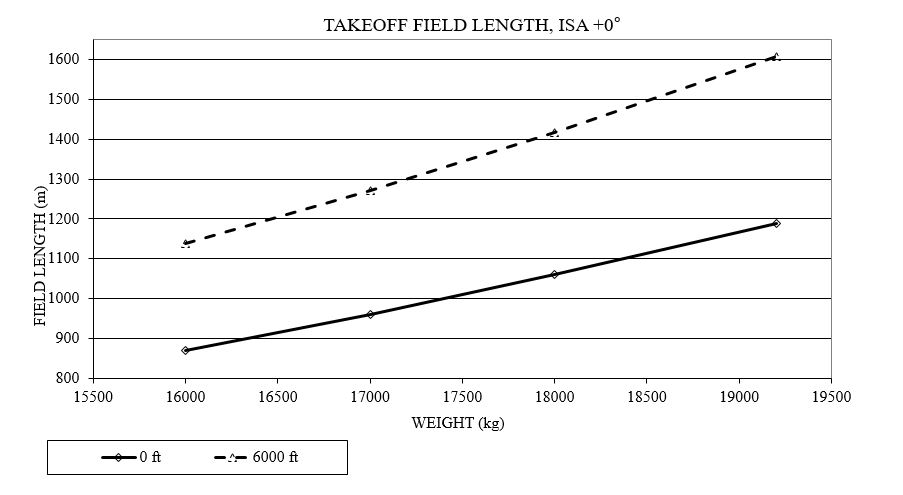
\includegraphics[width=1.\textwidth]{images/parte4/TOFL.JPG}
\caption{Comprimento de pista de decolagem}
\label{fig:tofl}
\end{figure}

\clearpage

\section{Pista de Pouso}

Para estimativa de pista de pouso, utilizou-se o modelo paramétrico proposto por \cite{lukaczyk2015suave} dado pela \autoref{eq:LFL}.


\begin{equation}
\label{eq:LFL}
    LFL = \sum_{i=0}^{2} k_i \cdot \left[ V_{app}^2 \right]^i
\end{equation}


\begin{table}[H]
    \centering
    \begin{tabular}{c|c c c}
        Wheel Trucks & $k_0$ & $k_1$ & $k_2$  \\ \toprule
         2 & 250 & 0 & 0.2533 \\
         4 & 250 & 0 & 0.3030 \\ \bottomrule
    \end{tabular}
    \caption{Coeficientes da \autoref{eq:LFL}}
    \label{tab:LFL}
\end{table}

A \autoref{fig:lfl} apresenta os resultados obtidos considerando apenas flaps como superfícies de sustentação, assim como na aeronave ATR 72-600, com uma deflexão de 15° e $C_{L_{max}} = 2.36$ para aeronave com trem de pouso extendidos.

\begin{figure}[H]
\centering
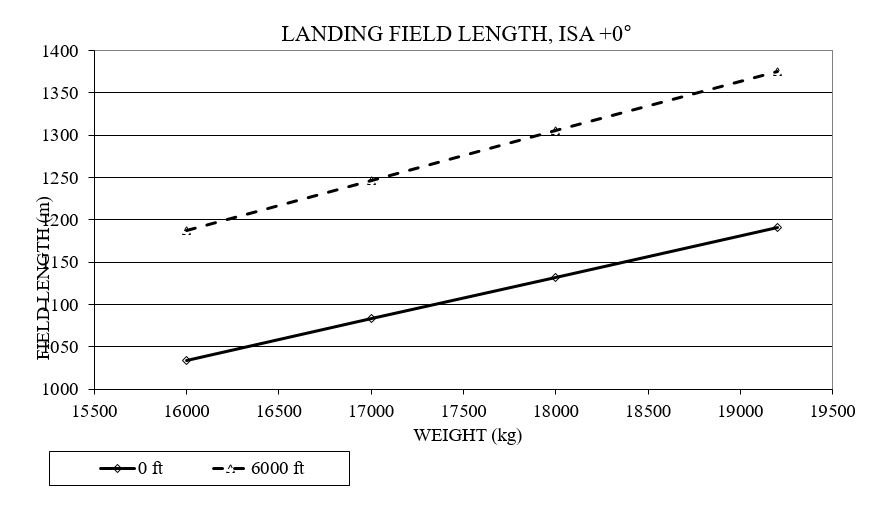
\includegraphics[width=1.\textwidth]{images/parte4/LFL.JPG}
\caption{Comprimento de pista de pouso}
\label{fig:lfl}
\end{figure}
